\section{Model methodologie}\label{Sect_Methodologie}
\subsection{Incurred but not reported}
	The task of the actuarial model is to predict the IBNR, the incurred but not reported claims. The IBNR can be divided into 3 distinct elements, which we defined as pure IBNR, IBNER and unpure IBNR. Pure IBNR are claims which are not reported at the observation date, meaning the insurer has no information on them. The insurer only knows that a claim happened. IBNER, incurred but not enough reported, are claims which have been reported and the insurer the information on the claims in their database. Unpure IBNR consist of claims which might reopen at any given time. This mean that a claim which closed in 2017 might reopen in 2018 or 2019. Unpure IBNR is a small proportion of the total IBNR, but still should be considered in the model. Figure XXX gives a visual representation of these categories. 
	\begin{figure}[H]
		\begin{center}
			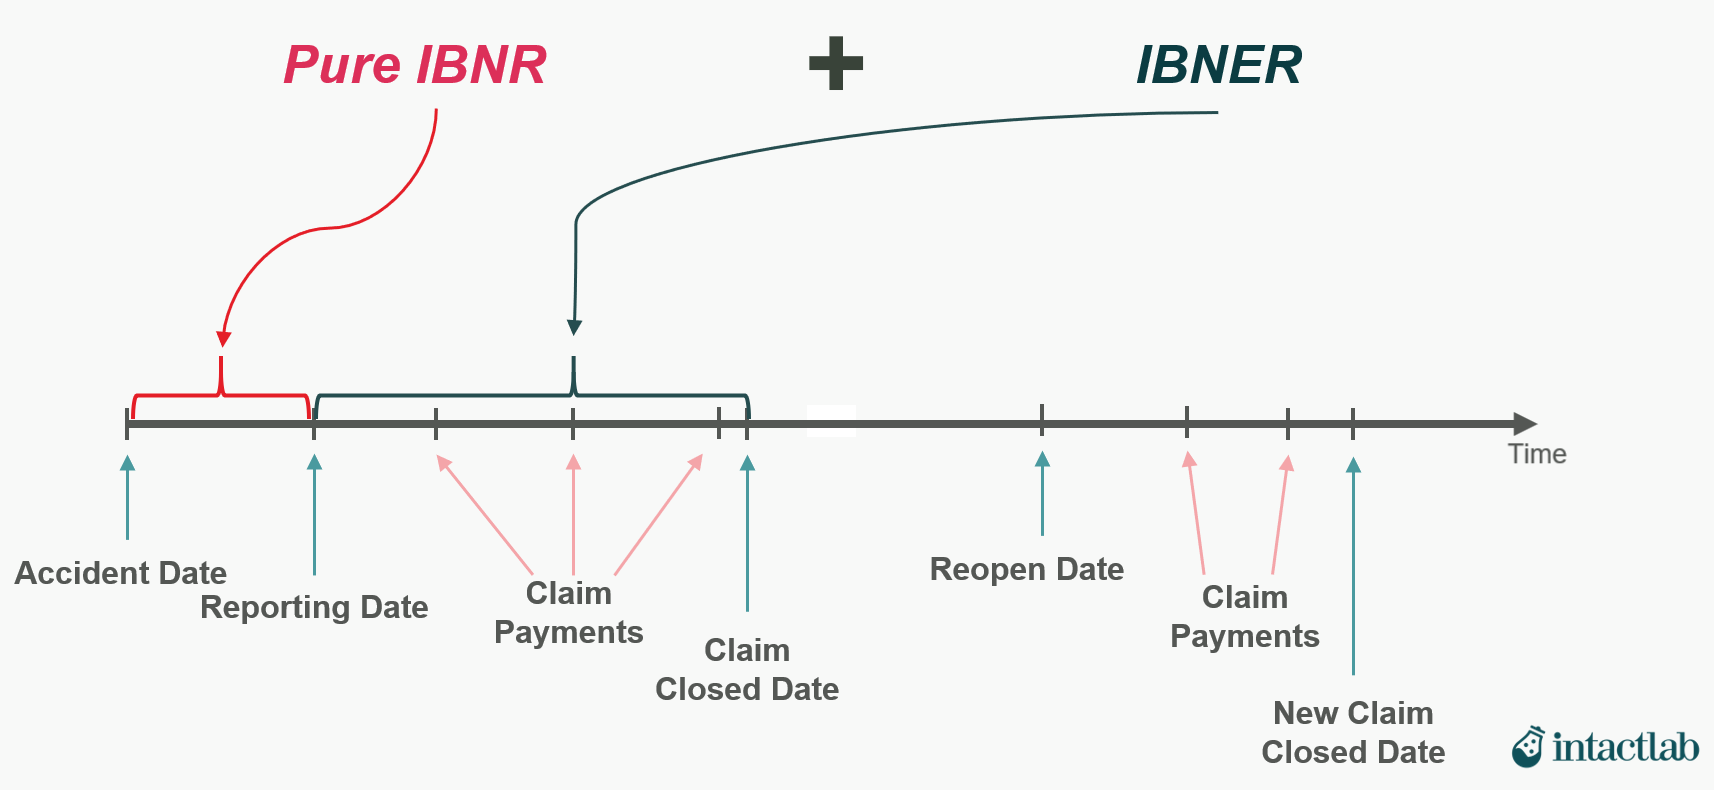
\includegraphics[scale=0.2]{Graphiques/IBNER_timeline} 
			\renewcommand{\figurename}{Figure}
			\caption{Timeline of a claim}\label{Fig_IBNER_timeline}
		\end{center}
	\end{figure}

\subsection{Hierarchical approach}
	The actuarial department uses a modified chain-ladder method for their model. We will try a more hierarchical approach, where we cluster our data in more homogeneous groups. First, we develop a model for each of the three IBNR types. Our team focuses on the IBNER part, while the pure and unpure IBNR models are still chain-ladder based and were developed by the actuarial department. For the IBNER model, we grouped the data according the following claims characteristics:  total loss, total loss without (\texttt{43}) replacement cost endorsement (\texttt{n43}), luxury repairable vehicles (\texttt{rep\_lux}), non luxury non rental repairable vehicles (\texttt{rep\_nlux\_nrent}) and non luxury rental repairable vehicles (\texttt{rep\_nlux\_rent}). We suppose that the frequency and severity distributions are very similar within these groups. Figure XXX gives an overview of the hierarchical approach.
	\begin{figure}[H]
		\begin{center}
			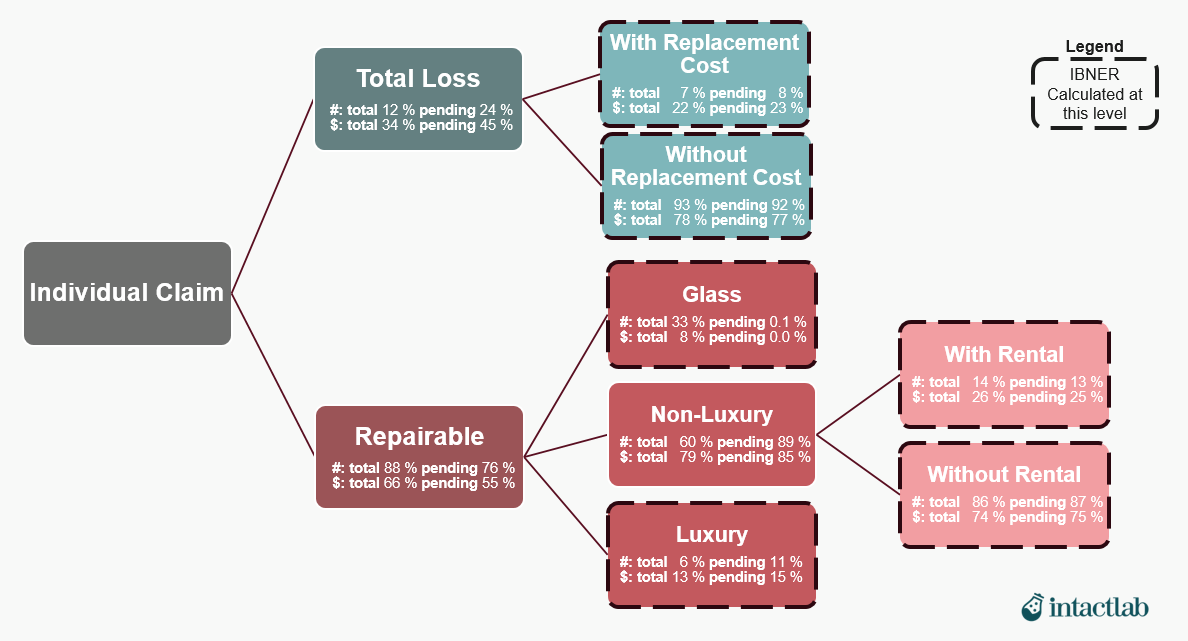
\includegraphics[scale=0.4]{Graphiques/Hier_model} 
			\renewcommand{\figurename}{Figure}
			\caption{Hierarchical model structure}\label{Fig_hier_model}
		\end{center}
	\end{figure}
 
\subsection{Key formulas}
	As mentioned in section ???, the ACV and GAV have strong predictive strength. We will use a basic formula to link the GAV/ACV with the ultimate and use historical observation on the pending (open) claims.

	 
	\begin{Definition}
		We define $\hat{L}_i$ as ultimate loss prediction for claims pending/open in period $i$ and $X_i$ as the predictor, in our case \texttt{GAV} or \texttt{ACV} used to predict period $i$. Their relationship is defined as
		$$\hat{L}_i = \hat{\Theta}_i \times X_i$$
		Where $\hat{\Theta}_i$ is the factor for time period $i$.
	\end{Definition}
	We need to calculate the factor $\hat{\Theta}_i$ with the available historical data. 
	\begin{Definition}
		We define $\widetilde{L}_{j,i}$ as total incurred for claims in time period $j$ as of $i$. $X_j$ is the predictor in time period $j$. Thus, the factor is defined as
		$$\hat{\theta}_i = \frac{\widetilde{L}_{j,i}}{X_j}$$
	\end{Definition}

	Note the difference between $\hat{L}_i$ and $\widetilde{L}_{j,i}$. The former is the ultimate we want to predict, so we do not know its value in observation month $i$. The latter is the total incurred for claims in period $j$ we know as of $i$. For illustration in the sample data of figure XXX and XXX, we want to calculate the factor $\hat{\theta}_{201804}$. We suppose we want to use open claim with $ \texttt{CLM\_NBR} = 123456789$ to calculate this factor, then 
	\begin{align*}
	\widetilde{L}_{201711, 201804} &= \texttt{AUTO\_LTD\_NET\_LOSS\_PAID\_AMT} + \texttt{AUTO\_LTD\_ALAE\_INCURRED\_AMT} \\
									& \ \ \	+ \texttt{AUTO\_LTD\_LOSS\_RES\_CHG\_AMT} \\
									&= 11213.87
	\end{align*}
	 as of $201804$ ($\texttt{obs\_month} = 201804$) and $X_j = \texttt{AvgTypicalCarValue} = 8007 $.
	As the example illustrated, the ultimate and the predictor are historical values which should be fully developed. It is necessary to have a least 5 to 12 months of development, so that the factors are stable enough. The difference in time between the moment we want to predict the pending and the historical data, $i - j$ is defined as the lag. How many historical observation month $j$ we use for the calculation is defined as period length. Figure XX shows a 5 months lag and 3 months period length. We want to predict the ultimate of the December 2018, $i = 201812$ pending (open) claims. We go back 5 months and use the historical claim data from open claims in May, June and July 2018, $j=201805, 201806, 201807$. 
	\begin{figure}[H]
		\begin{center}
			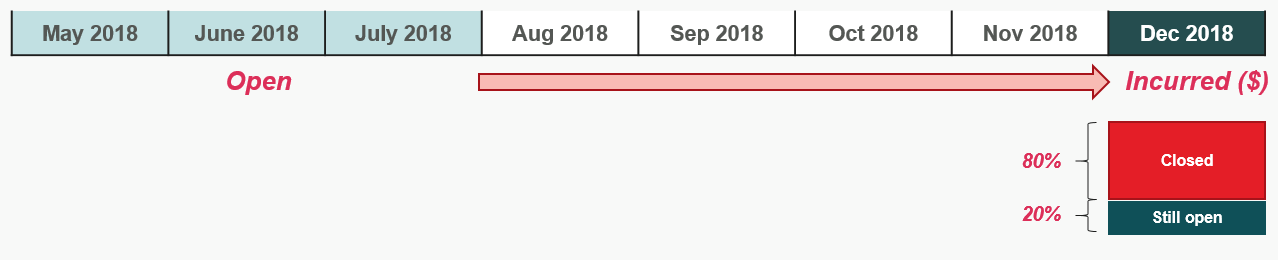
\includegraphics[scale=0.4]{Graphiques/lag_pl} 
			\renewcommand{\figurename}{Figure}
			\caption{Lag and period length visualization}\label{Fig_lag_pl}
		\end{center}
	\end{figure}
	This approach is similar to a lagged moving average model. We use the incurred as of December 2018 of claims open in May, June and July. Thus, the incurred had a minimum of 5 months to develop. Then, we divide this incurred by the aggregated GAV or ACV in May, June and July. We only keep the most recent data line for each claim, in other words we don’t have any duplicated per claim number. Figure XX gives a numerical example. 
	\begin{figure}[H]
		\begin{center}
			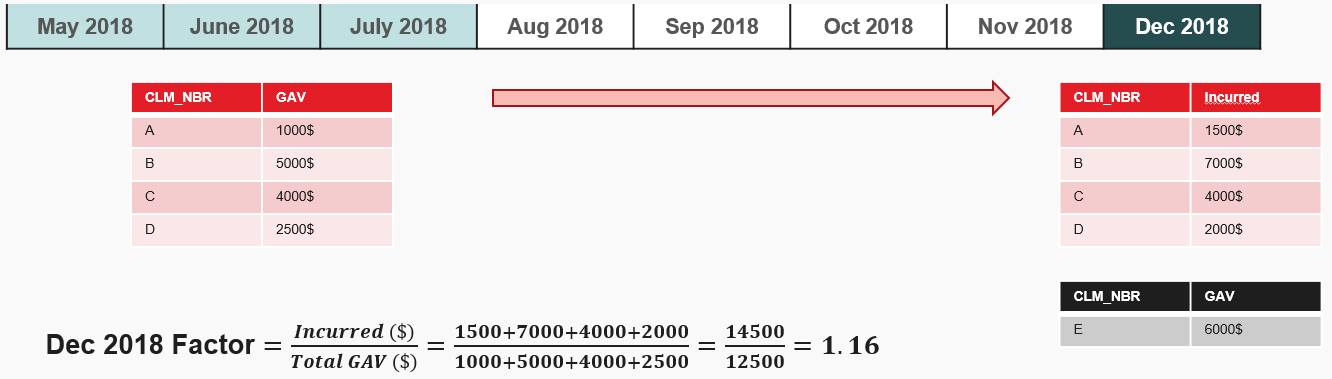
\includegraphics[scale=0.4]{Graphiques/factor_example} 
			\renewcommand{\figurename}{Figure}
			\caption{Factor calculation example}\label{Fig_factor_example}
		\end{center}
	\end{figure}
	Note that in figure \ref{Fig_lag_pl} the incurred is subdivided into open and closed claims, since it is possible that claims remain open even after 5 months. Therefore, we will calculate a claim number weighted average of closed and open factors. We get as final factor
	\begin{Definition}\label{Def_final_factor}
		$\hat{\Theta}_i$ is the final factor used for the prediction. $\hat{\theta}_{i,open}$ is the factor for claims that are still open during $i$ and  $\hat{\theta}_{i,closed}$ is the factor for claims that are closed during $i$. Furthermore, $n_{open}$ is the number of open claims in period $i$ and $n_{closed}$ is the number of closed claims in period $i$. Thus, we have
		$$\hat{\Theta}_i = n_{open} \hat{\theta}_{i,open} + n_{closed} \hat{\theta}_{i,closed}$$ 
	\end{Definition}
	
	We multiply this factor by the aggregated GAV or ACV of pending claims (December 2018 in our example) to get the ultimate amount.
	
	\begin{Definition}
		We define the $IBNER$ in period $i$ as
		$$IBNER_i = \hat{L}_i - I_i$$
		, where $I_i$ is the incurred payments and reserve for claims pending in period $i$.
	\end{Definition}
	Note that once claims are fully developed $L_i = I_i$, where $L_i$ is the real observed ultimate loss for claims open in period $i$. 
	The prediction results for the model will be discussed in section XX.
	
\subsection{Imputation methodology}
	It is important to note that no data is perfect. Our dataset contains a non negligible amount of missing GAV and ACV values. About 17\% of the claims have missing GAV or ACV, some regions and line of business are worse than others. Figure XX demonstrates how missing values are imputed. If we have missing values, we calculate the median of the existing values in the time window. We replace the missing values by the median and execute the factor calculations without any further readjustment. This method is not perfect and will be revised. For instance, in our example, we would overestimate the factor since we impute with a lower value.  
	\begin{figure}[H]
		\begin{center}
			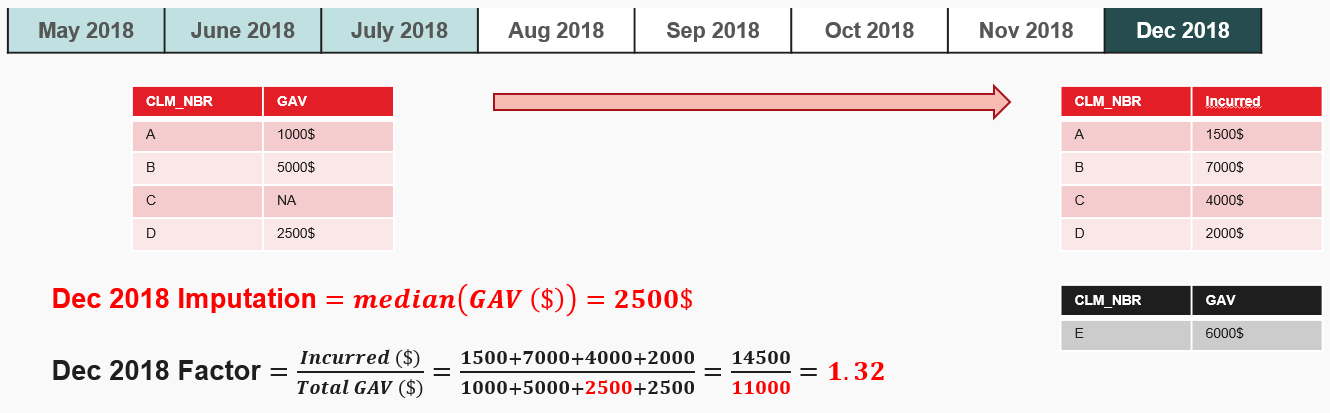
\includegraphics[scale=0.4]{Graphiques/imputation_example} 
			\renewcommand{\figurename}{Figure}
			\caption{Factor calculation example with missing values}\label{Fig_imputation_example}
		\end{center}
	\end{figure}

\subsection{Adjusting the lag and period length}
As we have noticed in the analysis of the data, Alberta clearly has different patterns than the other regions. Claims in Quebec and Ontario settle considerably faster (after 4-5 months) and recovery is less impactful. In Alberta having a lag of 5 is clearly insufficient, thus we will use a lag of 10. This gives the claims at least 10months to fully develop. In addition, a lag and period length that includes the 12th month, is beneficial if we have seasonal effects.
\subsection{Second model iteration: Historical pending but now closed claims}
After having used the first iteration of the model for January 2020. We noticed systematic error, constant over- or underestimations. This might be related to the open claims (after the lag) with are used to calculate the factors. Since open claims still have a case reserve the incurred used for the factor might be inflated, thus explaining overestimation. Indeed, the factor for open claims is always larger than the factor for closed. If we overestimate constantly, we attribute to much weight to still open claims. In the second iteration of the model we discard the weighted average and we only use the factor of closed claims. In short, based on definition \ref{Def_final_factor}, we have
$$\hat{\Theta}_i = \hat{\theta}_{i,closed}$$.
This also has the benefit that closed claims usually should not develop further and thus have less volatility in the calculation of the factors. The results will be discussed in section XXX.
\subsection{Third model iteration: Historical closed claims}
The final iteration of the model we will discuss in this report is based on the idea of the second iteration. We only want to use the factor of closed claims. However, in the second iteration we use the factor of closed claims of the lagged 3 month period, while in this iteration we want to increase the number of claims used in the calculations and add more recent claims. Consequently, instead of using the pending claims in a historical time window, we calculate factors for all claims that closed in the time window. This simply implies changing the filter on \texttt{sf\_status}. If we have use the previous example, we want to predict the pending claims in December 2018, we use all claims that closed between May and July for our factor calculations. Since the claims are closed it is unlikely that we have still open claims in December.
